\documentclass{article}
\usepackage[T1]{fontenc}
\usepackage{lmodern}
\usepackage{graphicx}
\usepackage{amsmath,amssymb}
\usepackage[a4paper,margin=2cm]{geometry}
\usepackage[absolute,overlay]{textpos}
\setlength{\TPHorizModule}{1mm}
\setlength{\TPVertModule}{1mm}
\usepackage[indonesian]{babel}
\usepackage{hyperref}
\setlength{\emergencystretch}{2em}
% unit: Halaman 24

\begin{document}

% === Halaman 24 (llm) ===

\vspace{193.05mm}

state
\vspace{50mm}
\[
\begin{bmatrix}
02 & 03 & 01 & 01 \\
01 & 02 & 03 & 01 \\
01 & 01 & 02 & 03 \\
03 & 01 & 01 & 02
\end{bmatrix} = \begin{bmatrix} [ \ ] \\
[ \ ] \\
[ \ ] \\
[ \ ]
\end{bmatrix}
\]

% deskripsi: Diagram transisi state yang menunjukkan dua matriks elemen 'a' untuk 'state' dan elemen 'b' untuk 'state\'' dengan panah yang menghubungkan mereka ke sebuah matriks numerik di bagian bawah.
% bbox normalisasi: [0.1800, 0.2100, 0.8100, 0.8600]
\begin{textblock*}{132.30mm}(37.80mm,62.37mm)
\noindent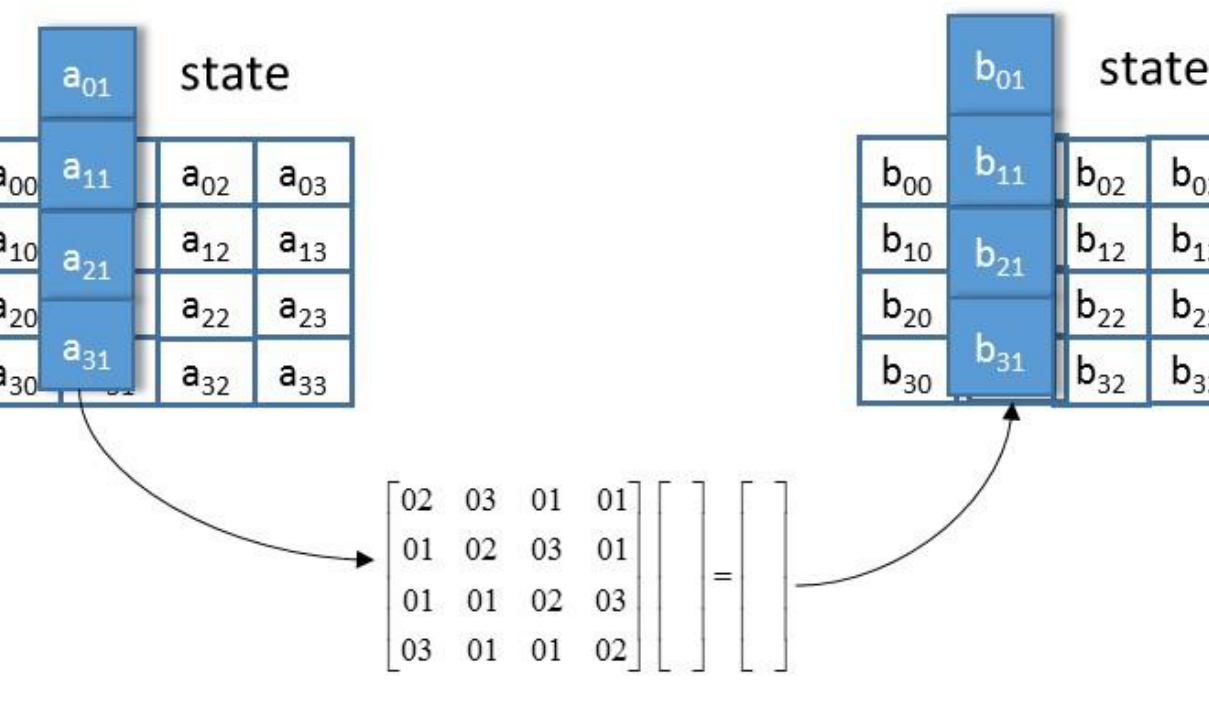
\includegraphics[width=132.30mm,height=193.05mm]{../../images/llm/page_024_img_01.png}%
\end{textblock*}

\end{document}
